\section{Цель работы}
Цель работы --- найти функцию, являющуюся наилучшим приближением заданной табличной функции по методу наименьших квадратов.
\section{Рабочие формулы используемых методов}
\begin{itemize}
	\item Метод наименьших квадратов для линейной функции:
	      \[
		      S_{XX} = \sum_{i=1}^n x_i^2
		      \quad
		      S_X = \sum_{i=1}^n x_i
		      \quad
		      S_Y = \sum_{i=1}^n y_y
		      \quad
		      S_{XY} = \sum_{i=1}^n x_i y_i
	      \]
	      \[
		      \Delta = n S_{XX} - S_X S_Y
		      \quad
		      \Delta_1 = n S_{XY} - S_X S_Y
		      \quad
		      \Delta_2 = S_{XX} S_Y - S_X S_{XY}
	      \]
	      \[
		      a = \Delta_1 / \Delta
		      \quad
		      b = \Delta_2 / \Delta
	      \]
\end{itemize}

\section{Вычислительная часть задачи}
\[
	y = \frac{17 x}{x^4 + 16}
	\qquad
	x \in [-4, 0], h = 0.4
\]

Табулирование данной функции представлено на~\cref{table:func_tabling}.

\begin{table}
  \caption{Табулирование функции}\label{table:func_tabling}
	\centering
	\begin{tabular}{rrr}
		\toprule
		\(i\) & \(x_i\) & \(y(x_i)\) \\
		\midrule
		1     & -4.0    & -0.2500    \\
		2     & -3.6    & -0.3327    \\
		3     & -3.2    & -0.4501    \\
		4     & -2.8    & -0.6145    \\
		5     & -2.4    & -0.8296    \\
		6     & -2.0    & -1.0625    \\
		7     & -1.6    & -1.2060    \\
		8     & -1.2    & -1.1287    \\
		9     & -0.8    & -0.8288    \\
		10    & -0.4    & -0.4243    \\
		11    & 0.0     & 0.0000     \\
		\bottomrule
	\end{tabular}
\end{table}

\subsection{Линейная аппроксимация}
\[
  S_X = -4 -3.6  -3.2  -2.8  -2.4  -2  -1.6  -1.2  -0.8  -0.4 + 0  = -22.0000
\]
\[
  S_{XX} = 
  16 + 12.96 + 10.24 + 7.84 + 5.76 + 4 + 2.56 + 1.44 + 0.64 + 0.16 + 0 = 61.6
\]
\begin{align*}
  S_Y &=
  (-0.2500) + (-0.3327) + (-0.4501) + (-0.6145) + (-0.8296) + (-1.0625) + \\ &+ (-1.2060) + (-1.1287) + (-0.8288) + (-0.4243) + (0.0000) = \\ &= -7.1272
\end{align*}

\begin{align*}
  S_{XY} &=
  1.0000 + 1.1976 + 1.4404 + 1.7205 + 1.9912 + 2.1250 + \\ &+ 1.9296 + 1.3545 + 0.6630 + 0.1697 + 0.0000 = \\ &= 13.5915
\end{align*}

\begin{align*}
  \Delta &= S_{XX} \cdot n - S_X \cdot S_X = 193.6 \\
  \Delta_1 &= n S_{XY} - S_X S_Y = -7.2928 \\
  \Delta_2 &= S_{XX} S_Y - S_X S_{XY} = -140.0250 \\
\end{align*}
\[
  a = \Delta_1 / \Delta = -0.0377 \qquad
  b = \Delta_2 / \Delta = -0.7233
\]

\begin{table}
  \caption{Вычисление среднеквадратичного отклонения}\label{table:std_linear}
  \centering
  \begin{tabular}{rrrrr}
    \toprule
    \(i\) & \(x_i\) & \(y_i\) & \(\varphi(x_i)\) & \({(\varphi(x_i) - y_i)}^2\) \\
    \midrule
    1 & -4.0 & -0.2500 & -0.5726 & 0.1041 \\
    2 & -3.6 & -0.3327 & -0.5877 & 0.0650 \\
    3 & -3.2 & -0.4501 & -0.6027 & 0.0233 \\
    4 & -2.8 & -0.6145 & -0.6178 & 0.0000 \\
    5 & -2.4 & -0.8296 & -0.6329 & 0.0387 \\
    6 & -2.0 & -1.0625 & -0.6479 & 0.1719 \\
    7 & -1.6 & -1.2060 & -0.6630 & 0.2949 \\
    8 & -1.2 & -1.1287 & -0.6781 & 0.2031 \\
    9 & -0.8 & -0.8288 & -0.6931 & 0.0184 \\
    10 & -0.4 & -0.4243 & -0.7082 & 0.0806 \\
    11 & 0.0 & 0.0000 & -0.7233 & 0.5231 \\
    \bottomrule
  \end{tabular}
\end{table}

Вычисление среднеквадратичного отклонения для линейной
аппроксимации представлено на~\cref{table:std_linear}.
Итоговое значение среднеквадратичного отклонения:
\[
  \delta = 0.3721
\]

\subsection{Квадратичная аппроксимация}

Значения \(S_X, S_{XX}, S_{Y}, S_{XY}\) взяты из предыдущего пункта.
Вычисления \(S_{XXX}, S_{XXXX}, S_{XXY}\) аналогичны предыдущем и опущены.

\[
  S_{XXX} = -193.6000
  \quad
  S_{XXXX} = 648.5248
  \quad
  S_{XXY} = -32.0779
\]

Построим СЛАУ для вычисления коэффициентов \(a_0, a_1, a_2\):
\( \mathbf{A} \mathbf{x} = \mathbf{b} \)
\[
  \mathbf{A} = \begin{pmatrix}
    n & S_X & S_{XX} \\
    S_X & S_{XX} & S_{XXX} \\
    S_{XX} & S_{XXX} & S_{XXXX}
  \end{pmatrix} =
  \begin{pmatrix}
    11 & -22 & 61.6 \\ 
    -22 & 61.6 & -193.6 \\
    61.6 & -193.6 & 648.5248
  \end{pmatrix}
\]
\[
  \mathbf{b} = \begin{pmatrix}
    S_Y \\
    S_{XY} \\
    S_{XXY}
  \end{pmatrix} =
  \begin{pmatrix}
    -7.1272 \\
    13.5915 \\
    -32.0779 \\
  \end{pmatrix}
\]

Решением данной системы является следующий вектор \(\mathbf{x}\):
\[
  \mathbf{x} = \begin{pmatrix}
    -0.1570 \\
    0.9062 \\
    0.2360
  \end{pmatrix}
\]

Таким образом, квадратичной аппроксимацией данной функции \(y(x)\)
является функция:
\[
  \varphi(x) = -0.157 + 0.9062 x + 0.2360 x^2
\]

Вычисление среднеквадратичного отклонения для данной функции
представлено на~\cref{table:std_quadratic}.
Итоговое значение среднеквадратичного отклонения \(\delta\):
\[
  \delta = 0.1652
\]

\begin{table}
  \caption{Вычисление среднеквадратичного отклонения для квадратичной аппроксимации}\label{table:std_quadratic}
  \centering
  \begin{tabular}{rrrrr}
    \toprule
    \(i\) & \(x_i\) & \(y_i\) & \(\varphi(x_i)\) & \({(\varphi(x_i) - y_i)}^2\) \\
    \midrule
    1 & -4.0 & -0.2500 & -0.0063 & 0.0594 \\
    2 & -3.6 & -0.3327 & -0.3611 & 0.0008 \\
    3 & -3.2 & -0.4501 & -0.6405 & 0.0362 \\
    4 & -2.8 & -0.6145 & -0.8443 & 0.0528 \\
    5 & -2.4 & -0.8296 & -0.9726 & 0.0204 \\
    6 & -2.0 & -1.0625 & -1.0255 & 0.0014 \\
    7 & -1.6 & -1.2060 & -1.0028 & 0.0413 \\
    8 & -1.2 & -1.1287 & -0.9046 & 0.0502 \\
    9 & -0.8 & -0.8288 & -0.7309 & 0.0096 \\
    10 & -0.4 & -0.4243 & -0.4817 & 0.0033 \\
    11 & 0.0 & 0.0000 & -0.1570 & 0.0246 \\
    \bottomrule
  \end{tabular}
\end{table}

\subsection{Вывод по вычислительной части}
Так как значение \(\delta\) для квадратичной аппроксимации меньше, то
эта функция является \emph{лучшей аппроксимацией}.
Графики функции \(y(x)\), линейной и квадратичной аппроксимации 
представлены на~\cref{fig:chart}.

\begin{figure}
  \centering
  \includegraphics[width=0.9\textwidth]{./img/chart.pdf}
  \caption{Графики аппроксимаций и исходной функции}\label{fig:chart}
\end{figure}

\section{Программная часть задачи}
\inputminted[breaklines]{Python}{../solution/solution.py}

\begin{center}
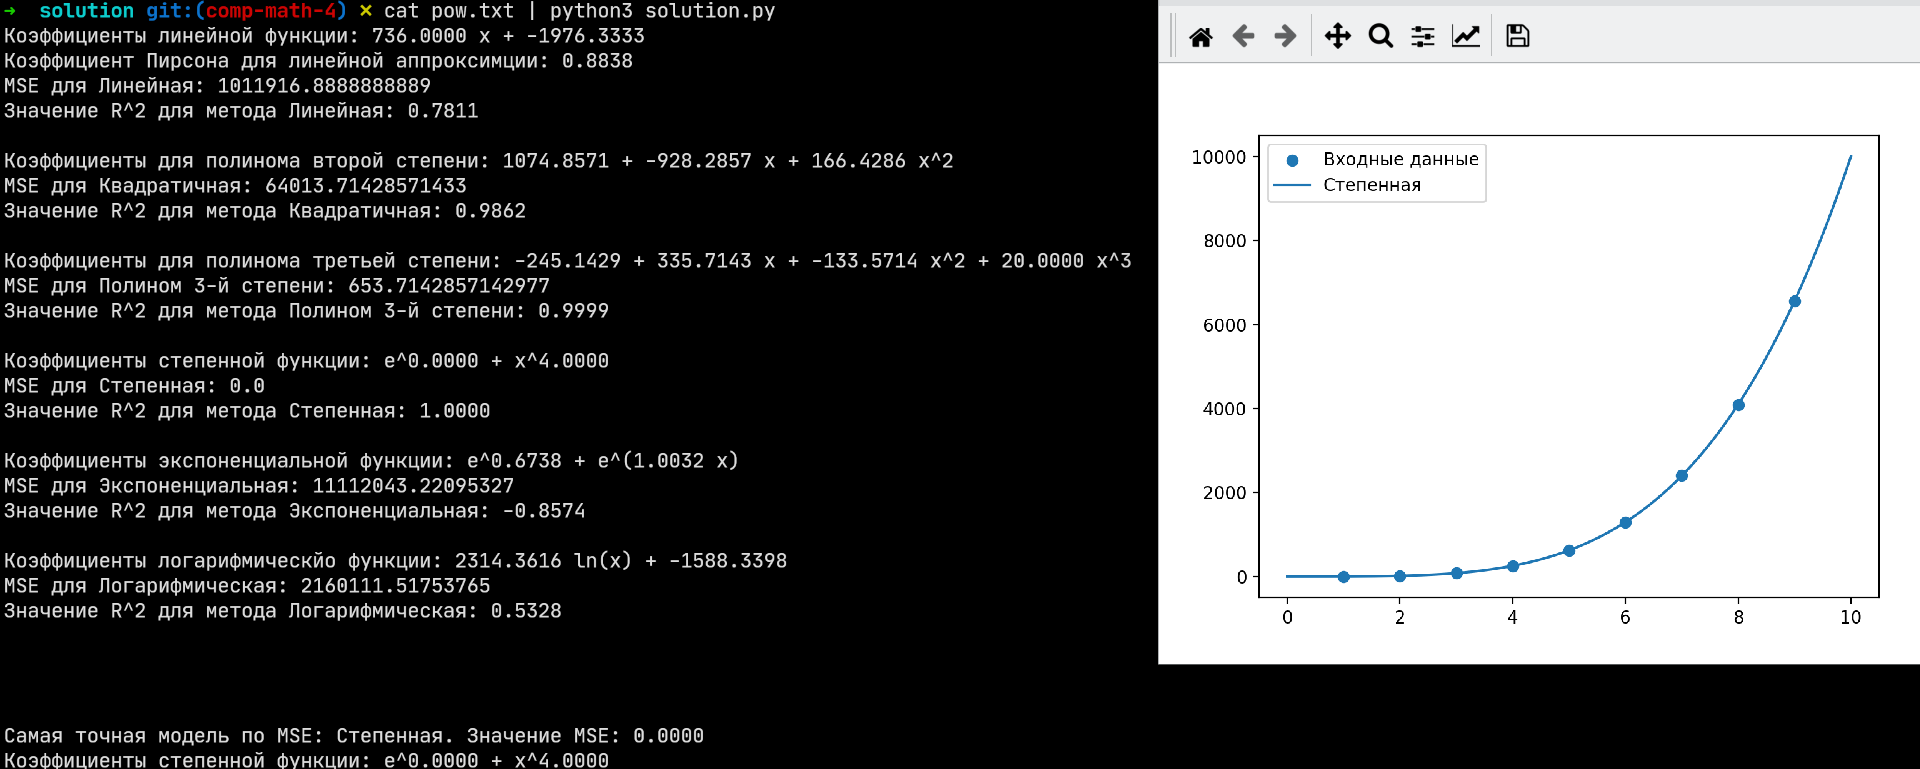
\includegraphics[width=0.9\textwidth]{./img/test1.png}
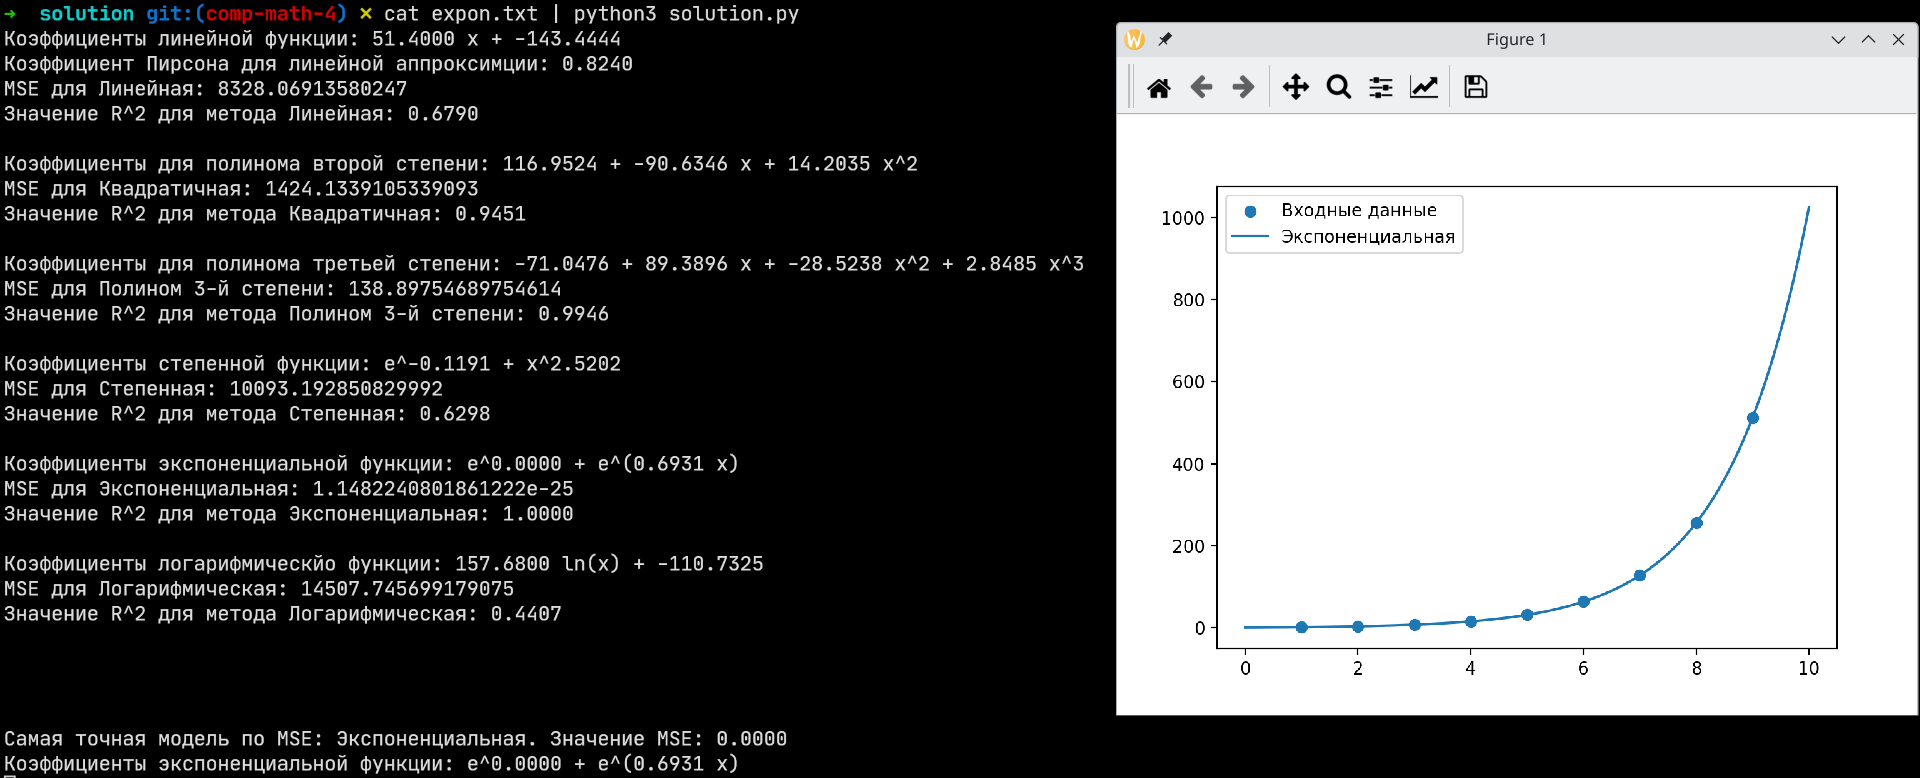
\includegraphics[width=0.9\textwidth]{./img/test2.png}
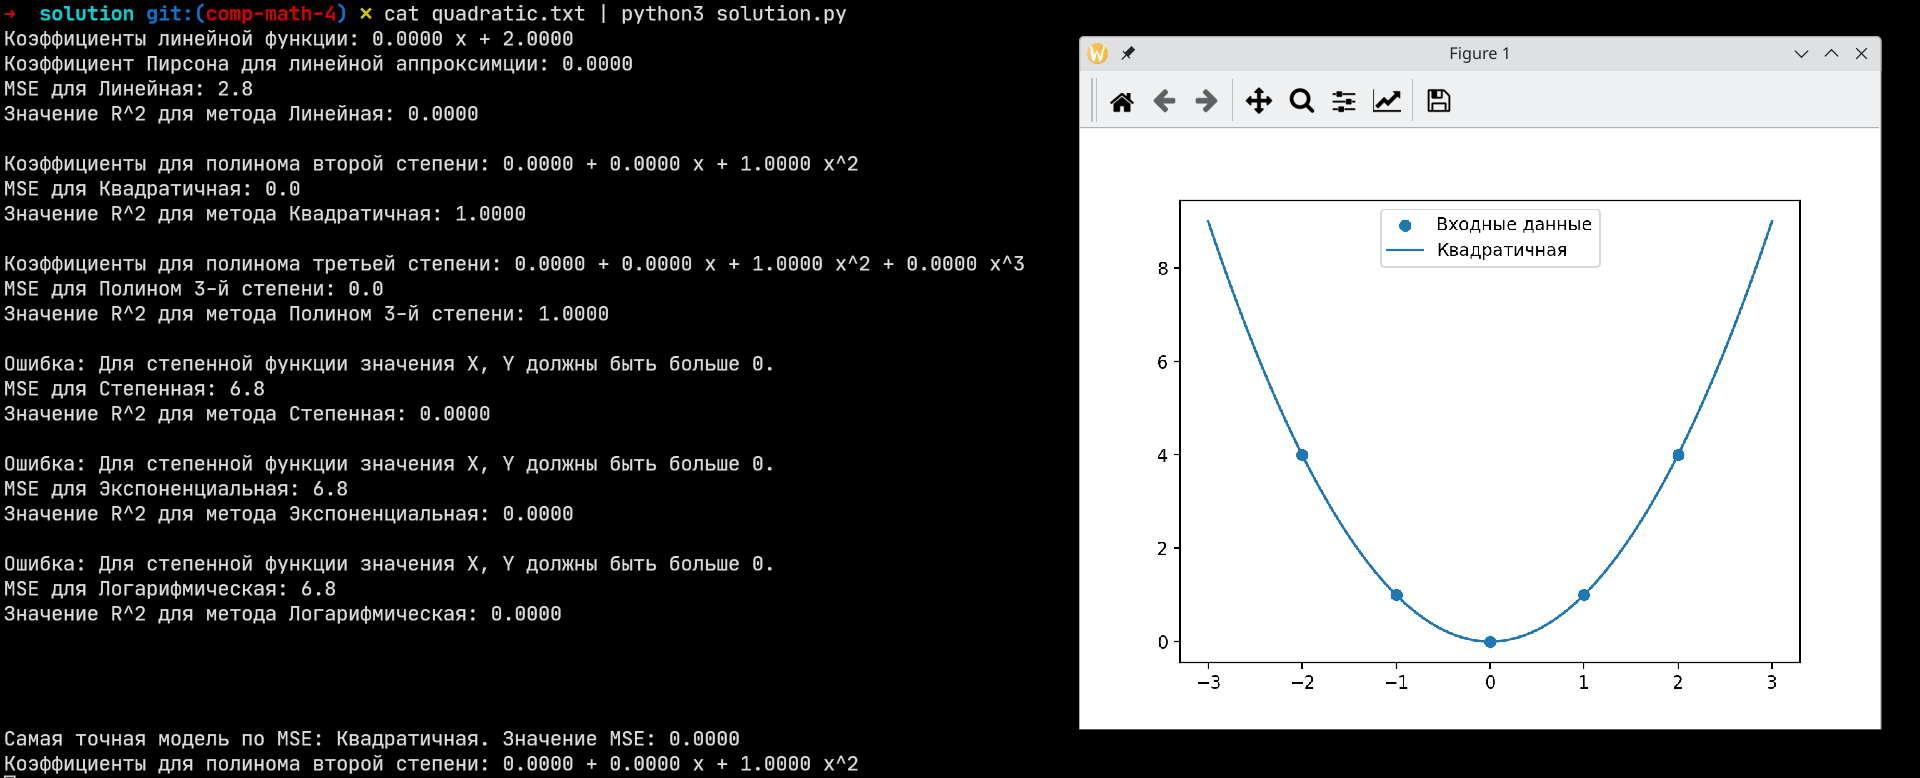
\includegraphics[width=0.9\textwidth]{./img/test3.png}
\end{center}

\section{Вывод}
В ходе выполнения данной лабораторной работы мною были изучены методы линейной
аппроксимации и методы полиномиальной аппроксиации.
Также мною были изучены методы сведения экспоненциальной, степенной и пр. аппроксимации
к линейной аппроксимации. Все эти методы были реализованы на языке Python.
